% Final Report (Due on 12/11/2025)

% Introduction, including a summary of the project, related work/methods, and the results of this project.

% Problem description, including a detailed description of the problem you address in this project.

% Methodology, including a detailed description on the methods you developed or used.

% Experiments, including, experiment setting, results, and your observations.

% Conclusion and future work, including a summary of the main contributions of this project and potential future directions.

\documentclass{article}

% if you need to pass options to natbib, use, e.g.:
%     \PassOptionsToPackage{numbers, compress}{natbib}
% before loading neurips_2021

% ready for submission
\usepackage[final]{neurips_2021}

% to compile a preprint version, e.g., for submission to arXiv, add add the
% [preprint] option:
%     \usepackage[preprint]{neurips_2021}

% to compile a camera-ready version, add the [final] option, e.g.:
%     \usepackage[final]{neurips_2021}

% to avoid loading the natbib package, add option nonatbib:
%    \usepackage[nonatbib]{neurips_2021}

\usepackage[utf8]{inputenc} % allow utf-8 input
\usepackage[T1]{fontenc}    % use 8-bit T1 fonts
\usepackage{hyperref}       % hyperlinks
\usepackage{url}            % simple URL typesetting
\usepackage{booktabs}       % professional-quality tables
\usepackage{amsfonts}       % blackboard math symbols
\usepackage{nicefrac}       % compact symbols for 1/2, etc.
\usepackage{microtype}      % microtypography
\usepackage{xcolor}         % colors
\usepackage{algorithm}
\usepackage{algpseudocode}
\usepackage{float}
\usepackage{amsmath}
\usepackage{graphicx}
\usepackage{subcaption}

\setlength{\textfloatsep}{8pt}
\setlength{\floatsep}{8pt}
\setlength{\intextsep}{6pt}

\title{Graph Coloring for Efficient Code Compilation}

% The \author macro works with any number of authors. There are two commands
% used to separate the names and addresses of multiple authors: \And and \AND.
%
% Using \And between authors leaves it to LaTeX to determine where to break the
% lines. Using \AND forces a line break at that point. So, if LaTeX puts 3 of 4
% authors names on the first line, and the last on the second line, try using
% \AND instead of \And before the third author name.



\author{
% I added our names in the style file. the stuff below doesnt work. btw the names are in alphabetical order. do we have a "first" author? - AE
% David S.~Hippocampus\thanks{Use footnote for providing further information
  %   about author (webpage, alternative address)---\emph{not} for acknowledging
  %   funding agencies.} \\
  % Department of Computer Science\\
  % Cranberry-Lemon University\\
  % Pittsburgh, PA 15213 \\
  % \texttt{hippo@cs.cranberry-lemon.edu} \\
  % examples of more authors
  Haven Cook \\
    RPI\\
  \texttt{cookh2@rpi.edu} \\
  \And
  Andrew Erickson \\ 
  RPI \\
  \texttt{ericka@rpi.edu} \\
  \And
  Ethan Rapa \\ 
    RPI \\
  \texttt{rapae@rpi.edu} \\
}

\begin{document}

\maketitle


\section{Introduction}
\subsection{Project Summary}

When examining possible ideas for this project, the group rallied around the idea of graph coloring, and the many applications therein. Eventually, we settled upon the application of graph coloring for register allocation in an x86 machine. After a diligent search, we found two promising datasets to use in this effort, but upon further investigation, neither could suit our needs. A broader discussion on these datasets is located in the "Related Work / Methods" section. We noticed a gap in the data that we needed and what was available so we decided to produce a dataset of interference graphs of a kind that, as far as we are aware, is novel and useful for ML researchers of this ilk. To accomplish this feat, we produced an automated Interference Graph generator utilizing LLVM and the Mem2Reg optimizer. LLVM generates readable intermediate representation (IR) file. An IR file is the data structure or code used internally by a compiler to represent source code in the form of Single Static Assignment (SSA), which can be thought of as a virtual register. An IR is designed to be conducive to further processing, such as optimization and translation; in our case use in the Mem2Reg optimizer. A "good" IR must be accurate – capable of representing the source code without loss of information and independent of any particular source or target language. We can use this knowledge to generate interference graphs from instruction datasets producing one of the only complete open source models for developing an interference graph dataset from provided example code. Our project, unlike the other datasets, also contends with so called Phi nodes. These nodes are used to uphold the SSA principle, which requires every variable to be assigned a value exactly once. In reality phi nodes are placed at the beginning of a block in an IR file, and are used to select a value depending on what the previous block was. 

For example:

\begin{verbatim}
block3:
    result = phi i32 [%a, %block1], [%b, %block2]    
\end{verbatim}

This means that if the previous block was block1, choose value a. If the previous block was block2, choose value b. This is done to prevent assigning the variable "result" in two different blocks such as an "if" block and an "else" block.

Our methodology produces interference graphs that accurately represent variable interference in real C programs, including those with multiple functions calling one another, and it does so up to 50x faster than previous works in the field. Its scalability allows it to efficiently process a dataset containing over 330,000 C files, and produces statistical analytics as the final stage of the pipeline.

The code is publicly available from https://github.com/A3dprintedman/DLOG-Project

\subsection{Related Work}

Two graph coloring datasets were procured but found to be unsubtle. The first one we found was the DIMACS graph coloring benchmark[15]. This dataset was created to profile the performance of existing heuristics based graph coloring models and other such graph coloring algorithms over an array of four problems. There are many problems with using this dataset for training. First of all, these graphs aren't interference graphs, nor are they derived from a compiled code. They are simply academic problems and aren't rooted in any practical register allocation tasks. They have the wrong structure, wrong chromatic profile, and no program semantics. Training on them would teach the model patterns that simply don’t exist in real compiler workloads. 

The second dataset we obtained was the RigSet Register Interference Graphs Dataset (Zaffalon 2024). This dataset was produced for training Machine Learning models focused on register allocation. It even contained PBQP interference graphs from real C/C++ codes. However, some limitations prevented us from choosing it. The graphs in RigSet are generated by doing a linear scan over the IR instead of analyzing true code dependencies. This involves finding the first time a variable is defined and the last time it is used, while not taking into account semantics such as blocking and non-linear jumps. As a result, the generated graphs do not properly simulate compiler register partitioning through interference graph generation. Our work directly fixes both problems; we generate interference graphs by considering all non-linear paths. Our graphs reflect real liveliness, real control flow, and real register pressure. Using high-performance techniques and low-level C methods, our graph generator also operates orders of magnitude faster than previous implementations. 

\section{Methods}

Register allocation can be redefined as a graph coloring problem. As a result, optimal solutions to the register allocation problem is NP-complete (Collberg 2011). The graph that must be colored can be modeled as an interference graph $G = (V, E)$, where $G$ is an undirected graph where the nodes are variables that require a register, and thus can be placed in a \textit{virtual register} $N = \{N_1, N_2, \ldots, N_n\}$ of length $n$ in which $\forall\, n \in \{1,\ldots,\mathbb{N}_{\ge 1}\}$. Virtual register convention enforces two rules: (i) the virtual register may only ever hold a single variable during its lifespan, and there is no spilling, and (ii) virtual register allocation is infinite. 

The LLVM compiler can generate intermediate representation (IR) static single-assignment form (SSA) files, or abstracted machine code used for compiler development. By using mem2reg conversion, memory references in the generated file can be treated as virtual registers (Lattner and Atne 2004). Furthermore, we have access to non-sequential labels such as branches and phi nodes. IR files divide sequential and non-sequential operations using blocks. Liveness becomes a tree traversal operation where nodes are blocks. \textbf{Figure \ref{fig:livenessofIR}} demonstrates how to parse an IR file when comparing block and instruction-level granularity. 

Graph interference can be cast as a hierarchical liveness problem (Rastello and Tichadou 2022; Collberg 2011). Let $\textit{USE}[K]$ represent variables whose values are being used before being assigned to in $K$, where $K \in \{I,B\} $, or block and instruction. Let $\textit{DEF}[K]$ represent variables whose values are being assigned before being used in $K$. If we understand when a virtual register is being used and defined at both the instruction and block levels, we can ultimately track when a variable is live while entering ($\textit{IN}[B]$) or leaving ($\textit{OUT}[B]$) a block. We refer to the structure of \textbf{figure \ref{fig:livenessofIR}} as a directed \textit{Control Flow Graph (CFG)}.

Therefore, we define the steps of interference graph generation as follows: (i) compile code into an IR file using LLVM, (ii) compute $\textit{USE}[K]$ and $\textit{DEF}[K]$, (iii) account for changes in $\textit{USE}[B]$ and $\textit{DEF}[B]$ given $\phi$, (iv) compute $\textit{IN}[B]$ and $\textit{OUT}[B]$ using an iterative data flow algorithm, (v) build an interference graph while treating functions as an independent set, (vi) recursively account for the caller-callee function paradigm by treating ancestor functions as super nodes. 

\begin{figure}[ht]

    \centering
    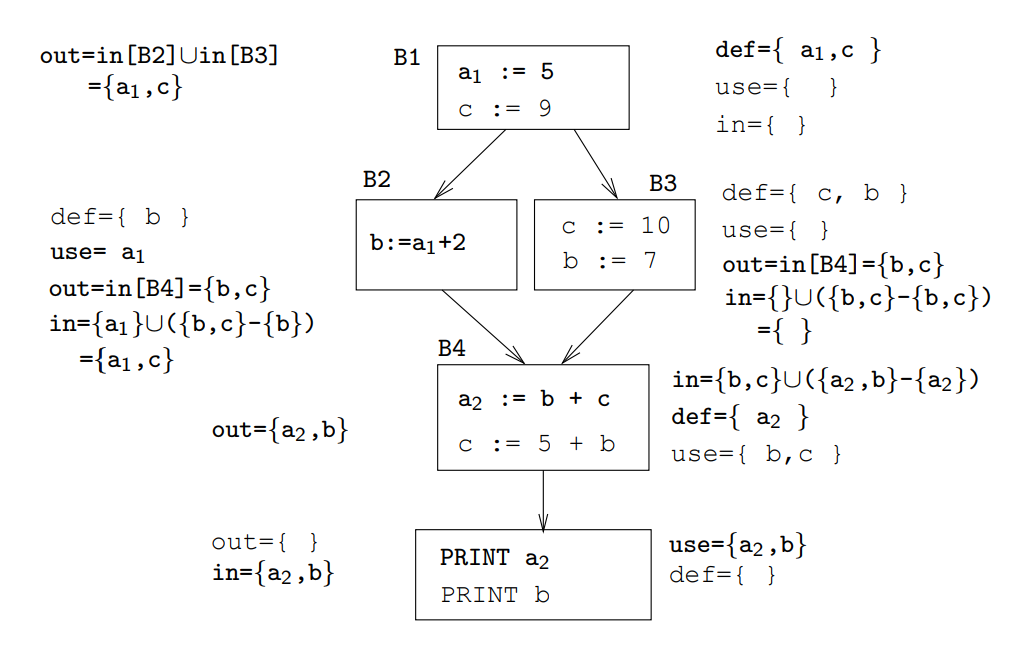
\includegraphics[width=1\linewidth]{figures/liveness_example.png}
    \caption{Computing $\textit{USE}[K]$, $\textit{DEF}[K]$, $\textit{IN}[B]$, and $\textit{OUT}[B]$ across all blocks in an IR file}
    \label{fig:livenessofIR}
    
\end{figure}

We designed a high-throughput compilation pipeline that parallelizes compiling the necessary IR file and generates, generates the output edge list, and produces helpful statistics about total graph features such as average edges and vertices, and visuals showing distribution of graph degrees and the chromatic number discovered for the graph. \textbf{Figure \ref{fig:workflow}} outlines this workflow. 

\begin{figure}[ht]

    \centering
    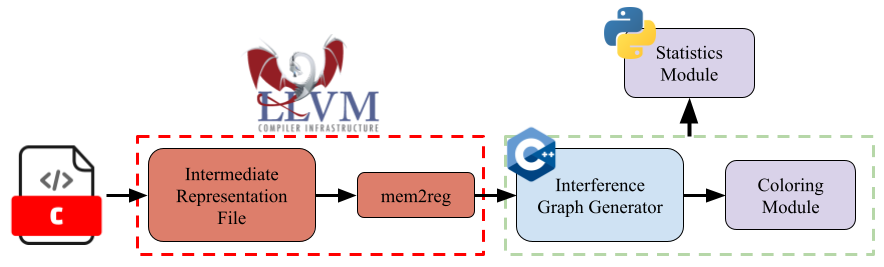
\includegraphics[width=1\linewidth]{figures/Workflow.png}
    \caption{Automated workflow of interference graph generator}
    \label{fig:workflow}
    
\end{figure}

\subsection{Liveness Tracking}

After generating an IR file that uses SSA, state machines extract the necessary tokens, first allocating sized data structures, and then populating $\textit{DEF}[I]$ / $\textit{USE}[I]$ given the left and right-hand side elements. During this time, a block's successors and predecessors are tracked, given any switch, branch, or  $\phi$-node tokens. An abstraction of virtual register use and definitions to per-block tracking is necessary to compute liveness along block edges, given successors and predecessors. We can compute this new $\textit{DEF}[B]$ / $\textit{USE}[B]$ using the lemma that a virtual register found in use without first encountering a def must indicate the virtual register was defined outside the block. Any external uses must be added to $\textit{USE}[B]$, and in-block defines must be added to $\textit{DEF}[B]$. \textbf{Algorithm \ref{alg:perblock-usedef}} describes the implementation of this using a bitset to maintain best spatial locality. All block-level register activity was tracked using a bitset. 

SSA is limited in runtime computation representation. When control flow merges, a variable may become conditional. Since virtual registers cannot be redefined, LLVM instead flags these regions using $\phi$-nodes with register-predecessor pairs $[r, B]$, where $r$ is the register label. $\textit{DEF}[B]$ / $\textit{USE}[B]$ must be updated to account for unlabeled use and def only indicated by the $\phi$-node asserting liveness of the virtual register in the predecessor block. An example would be if the predecessor block does not define the virtual register or use it, but the successor indicates the virtual register is live in the block with a $\phi$-node, we must assume the virtual register is defined $B_t$ blocks up the predecessor tree while being live in all successors before the $\phi$-node. \textbf{Algorithm \ref{alg:phi-usedef}} is similar to \textbf{Algorithm \ref{alg:perblock-usedef}}, but recomputes predecessor $\textit{USE}[I]$ given the $\phi$ tokens discovered. 

\begin{algorithm}[H]
\label{alg:useordef}
\caption{Per-Block Use/Def}\label{alg:perblock-usedef}
\begin{algorithmic}[1]
\Require For each instruction $I$, sets $\mathrm{use}(I)$ and $\mathrm{def}(I)$
\Ensure For each block $b$, sets $\mathrm{use}(b)$ and $\mathrm{def}(b)$
\ForAll{basic blocks $b$ in the function}
    \State $\mathrm{use}(b) \gets \emptyset$
    \State $\mathrm{def}(b) \gets \emptyset$
    \For{$i \gets 1$ to $\#\mathrm{instr}(b)$}
        \State $I \gets \mathrm{instr}(b)[i]$
        \ForAll{$r \in \mathrm{use}(I)$}
            \If{$r \notin \mathrm{def}(b)$}
                \State $\mathrm{use}(b) \gets \mathrm{use}(b) \cup \{r\}$
            \EndIf
        \EndFor
        \ForAll{$r \in \mathrm{def}(I)$}
            \State $\mathrm{def}(b) \gets \mathrm{def}(b) \cup \{r\}$
        \EndFor
    \EndFor
\EndFor
\end{algorithmic}
\end{algorithm}

\begin{algorithm}[H]
\caption{Phi Uses (Predecessor Folding)}\label{alg:phi-usedef}
\begin{algorithmic}[1]
\Require $\phi$-nodes with operand–predecessor pairs $(r,p)$
\Ensure Block-level $\mathrm{use}(p)$ updated for $\phi$ operands
\ForAll{blocks $b$}
    \ForAll{$\phi \in \mathrm{phis}(b)$}
        \ForAll{$(r,p) \in \phi$}
            \If{$r \notin \mathrm{def}(p)$}
                \State $\mathrm{use}(p) \gets \mathrm{use}(p) \cup \{r\}$
            \EndIf
        \EndFor
    \EndFor
\EndFor
\end{algorithmic}
\end{algorithm}

The precursor to constructing an interference graph is computing a control flow graph (CFG), which describes the active virtual registers entering and exiting $B$ given the known in and out-block definitions: $\textit{DEF}[B]$ and $\textit{USE}[B]$. Iterative dataflow explores each path while transferring information to the predecessors about the liveness of virtual registers defined in the block. Virtual register calls in successor blocks must be communicated to the predecessor, forcing that virtual register to remain active after exiting the block. \textbf{Algorithm \ref{alg:liveliness}} outlines the \textit{liveliness algorithm} for final control flow computation. The total precompute time approaches worst-case $\Theta(I + BIR + B^2)$, where $R$ is the average number of virtual registers per line and $I$ is the number of instructions per block $B$. 

\begin{algorithm}[H]
\caption{Liveliness Algorithm}\label{alg:liveliness}
\begin{algorithmic}[1]
\Require Control-flow graph $CFG = (N, E)$
\Ensure Live-in and live-out sets $\textit{IN}[n]$, $\textit{OUT}[n]$ for all $n \in N$

\ForAll{$n \in B$}
    \State $\textit{IN}[n] \gets \emptyset$
    \State $\textit{OUT}[n] \gets \emptyset$
\EndFor

\Repeat
    \ForAll{$n \in B$}
        \State $\textit{IN}'[n] \gets \textit{IN}[n]$
        \State $\textit{OUT}'[n] \gets \textit{OUT}[n]$
        
        \State $\textit{OUT}[n] \gets \!\!\bigcup_{s \in \mathrm{succ}(n)}\!\! \textit{IN}[s]$
        \State $\textit{IN}[n] \gets \mathrm{use}[n] \cup \left(\textit{OUT}[n] \setminus \mathrm{def}[n]\right)$
    \EndFor
\Until{$\forall n \in N:\ \textit{IN}'[n] = \textit{IN}[n] \land \textit{OUT}'[n] = \textit{OUT}[n]$}

\end{algorithmic}
\end{algorithm}

When treating interference graph generation across functions as an independent task, we can use a modified form of Chaitin's Algorithm compatible with intermediate representation (Collberg 2011). \textbf{Algorithm \ref{alg:iggen}} describes this procedure and shows how liveness is a reverse process that must maintain global information about how exiting, traversing, and entering each block modifies instruction liveness. Edges are generated as $E \gets E \cup \{(\ell, d)\}$, where $\ell$ are the virtual registers currently in the active set at step $t$, and $d$ is a virtual register defined at that instruction. Liveness is updated using two rules: (i) a variable is live after an instruction and not killed with def, and (ii) the variable is used at the instruction. (i) is solved because we are using SSA, which will not allow redefinitions. It would be better to simplify $\textit{live} \gets \mathrm{use}(I) \cup (\textit{live} - \mathrm{def}(I))$ to $\textit{live} \gets \mathrm{use}(I) \cup (\textit{live})$, but both evaluate the same result. 

In order to store interference information about a function that accurately reflects how registers interfere across function calls, an extension of a typical edge list is utilized. In addition to adjacency information within the function's subgraph representing its variables, some variables will be live during a function call and, as such, are live during the entire execution of callee. To reconstruct a function's interference graph that contains it's entire call chain, an additional array is stored that contains the ID of each function called, and a corresponding list of every variable that is live across said call. Importantly, these function calls contain their own interference subgraph that is treated as an abstract building block. This means that a function can be called multiple times with different live variables depending on each instances context.

\begin{algorithm}[H]
\caption{Building an Interference Graph While Treating Functions as an Independent Set}\label{alg:iggen}
\begin{algorithmic}[1]
\Require Basic blocks $B$ with instruction lists; live-out sets $\textit{OUT}[b]$; per-instruction $\mathrm{use}(I)$ and $\mathrm{def}(I)$
\Ensure Interference graph $G = (V, E)$

\State $E \gets \emptyset$
\ForAll{$b \in B$}
    \State $\textit{live} \gets \textit{OUT}[b]$
    \ForAll{instructions $I \in b$ in reverse order}
        \ForAll{$d \in \mathrm{def}(I)$}
            \ForAll{$\ell \in \textit{live} \cup \mathrm{def}(I)$}
                \If{$\ell \neq d$}
                    \State $E \gets E \cup \{(\ell, d)\}$ \Comment{add interference edge}
                \EndIf
            \EndFor
        \EndFor
        \State $\textit{live} \gets \mathrm{use}(I) \cup (\textit{live} - \mathrm{def}(I))$
    \EndFor
\EndFor
\State \Return $G = (V, E)$
\end{algorithmic}
\end{algorithm}

\subsection{Recursive Interference}
Upon completion of \textbf{Algorithm \ref{alg:iggen}}, a shallow interference graph representation of the function it is called upon will have been populated. In general, this shallow graph is constructed for each function contained within the file. When processing a C file that contains multiple functions that call each other, it is more accurate to expand this subgraph using the function calls and their interferences. In order to do this, \textbf{Algorithm \ref{alg:recursively-populate}}, a recursive expansion procedure, was designed. The algorithm is divided into three stages: local interference addition, ancestral interference addition, and callee recursion. Additionally, a stack data structure was implemented that kept references to the interference information of the local function's ancestral call chain. The first stage involves appending the resultant edge list with the edges within the called function's subgraph. After this, the stack is iterated through, and each ancestor of the local function contributes its interfering variables as super-nodes of the local function's entire subgraph. Put more simply, every vertex in the local subgraph contributes an additional edge with each interfering variable across its entire ancestry. Finally, the local extended edge list data structure has its callee function array iterated through. In two cases, no recursive call is made upon a callee. If there is no interference subgraph created and stored for the function, which happens in externally linked libraries, or if the callee is the same function as the caller, i.e. recursion. In either case, no true adjacency information is contributed, but the functions and their interference are stored in the resultant extended edge list. Otherwise, the local function's interference information for the callee is pushed to the stack, and the recursive call is made.

\begin{algorithm}[H]
\caption{\textsc{RecursivelyPopulate}}
\label{alg:recursively-populate}
\begin{algorithmic}[1]

\Procedure{RecursivelyPopulate}{$\mathcal{L}, E, \text{prev}, f, \Delta, N, S$}

    \Statex \textbf{Stage 1: Add local interference edges}
    \For{$(u,v) \in \mathcal{L}[f].\text{Edges}$}
        \If{$S.\text{depth} \neq -1$}
            \State $E \gets E \cup \{(u+\Delta,\; v+\Delta)\}$
        \EndIf
    \EndFor

    \Statex \textbf{Stage 2: Interference with ancestor call chain}
    \For{$i = 0$ to $S.\text{depth}$}
        \For{$u \in S[i].\text{Neighbors}$}
            \For{$v = \Delta$ to $\Delta + \mathcal{L}[f].\text{NumVertices}-1$}
                \State $E \gets E \cup \{(u + S[i].\text{Offset},\; v)\}$
            \EndFor
        \EndFor
    \EndFor

    \State $\Delta \gets \Delta + \mathcal{L}[f].\text{NumVertices}$

    \Statex \textbf{Stage 3: Recurse into callees}
    \For{each call $c \in \mathcal{L}[f].\text{Calls}$}
        \State $g \gets \textsc{FindFunc}(\mathcal{L}, c.\text{FuncID}, N)$
        \If{$g = -1$ \textbf{or} $f = \text{prev}$} \Comment{Function information not found/recursion break}
            \State $E \gets E \cup \{(c.\text{FuncID},\; c.\text{Neighbors}+\Delta)\}$
        \Else
            \State $S.\text{Push}(c.\text{Neighbors},\; \Delta)$
            \State \Call{RecursivelyPopulate}{$\mathcal{L}, E, f, g, \Delta, N, S$}
        \EndIf
    \EndFor

    \State $S.\text{Pop}()$

\EndProcedure

\end{algorithmic}
\end{algorithm}

The conclusion of this algorithm yields a fully expanded interference graph for a function. Within our framework, there are a few different steps that can be taken afterward. First, utilizing \textbf{Algorithm \ref{alg:greedy-color}}, we implemented a simple serial greedy coloring algorithm that will translate the edge list to compressed sparse row form, and subsequently yield an array of colors corresponding to each vertex, as well as the chromatic number, $\chi$.

\begin{algorithm}[H]
\caption{\textsc{GreedyColor}}
\label{alg:greedy-color}
\begin{algorithmic}[1]

\Procedure{GreedyColor}{$G = (V,E)$}
    \State Initialize array $\text{Color}[v] \gets \text{UNCOLORED}$ for all $v \in V$

    \For{each vertex $v$ in the chosen order}
        \State Initialize set $U \gets \emptyset$      \Comment{Colors used by colored neighbors}

        \For{each neighbor $u$ of $v$}
            \If{$\text{Color}[u] \neq \text{UNCOLORED}$}
                \State $U \gets U \cup \{\text{Color}[u]\}$
            \EndIf
        \EndFor

        \State $c \gets 0$
        \While{$c \in U$}
            \State $c \gets c + 1$
        \EndWhile

        \State $\text{Color}[v] \gets c$     \Comment{Assign smallest feasible color}
    \EndFor

    \State \Return Color
\EndProcedure

\end{algorithmic}
\end{algorithm}

Post-coloring, the entire extended edge list can be exported to a file for external processing.

The final stage of the pipeline is a graph analysis tool written in Python. It parses the contents of an arbitrary number of output files and yields a set of user defined statistics.

\section{Results}

In order to demonstrate the scalability of this pipeline, the FormAI dataset containing 331,000 compilable C files was utilized. Due to certain library dependencies expected by some of the files in this dataset, graphs were generated for 215,819 of these, comprising both shallow and recursed interference graphs of 749,691 functions. Each of these files was compiled to LLVM intermediate representation, then processed and output to a file by the executable, and finally, the analysis was run on these outputs to determine several key statistics. 

\begin{figure}[ht]
    \centering
    \begin{subfigure}{0.48\linewidth}
        \centering
        
\includegraphics[width=\linewidth]{figures/chi.png}
        \caption{Distribution of Chromatic Numbers across functions in FormAI C dataset}
        \label{fig:chi}
    \end{subfigure}
    \hfill
    \begin{subfigure}{0.48\linewidth}
        \centering
        
\includegraphics[width=\linewidth]{figures/eoverv.png}
        \caption{Distribution of Average Degrees across functions in FormAI C dataset}
        \label{fig:eoverv}
    \end{subfigure}
    \caption{Structural properties of interference graphs in the FormAI C dataset}
\end{figure}

Analyzing the computational efficiency of our executable, a flame graph is produced on a sample C file. The transition from regex-based tokenization to c-style state machine tokenization resulted in a performance increase of over 50x with sanitizers still enabled. \textbf{Figure \ref{fig:flamegraph}} shows there are still optimizations that can be made: fileIO buffer manipulation and a transition to hashing in C over stl C++ are the largest candidates. Precomputing and reading lines from the file could also be multithreaded.

\begin{figure}[htbp]
    \centering
    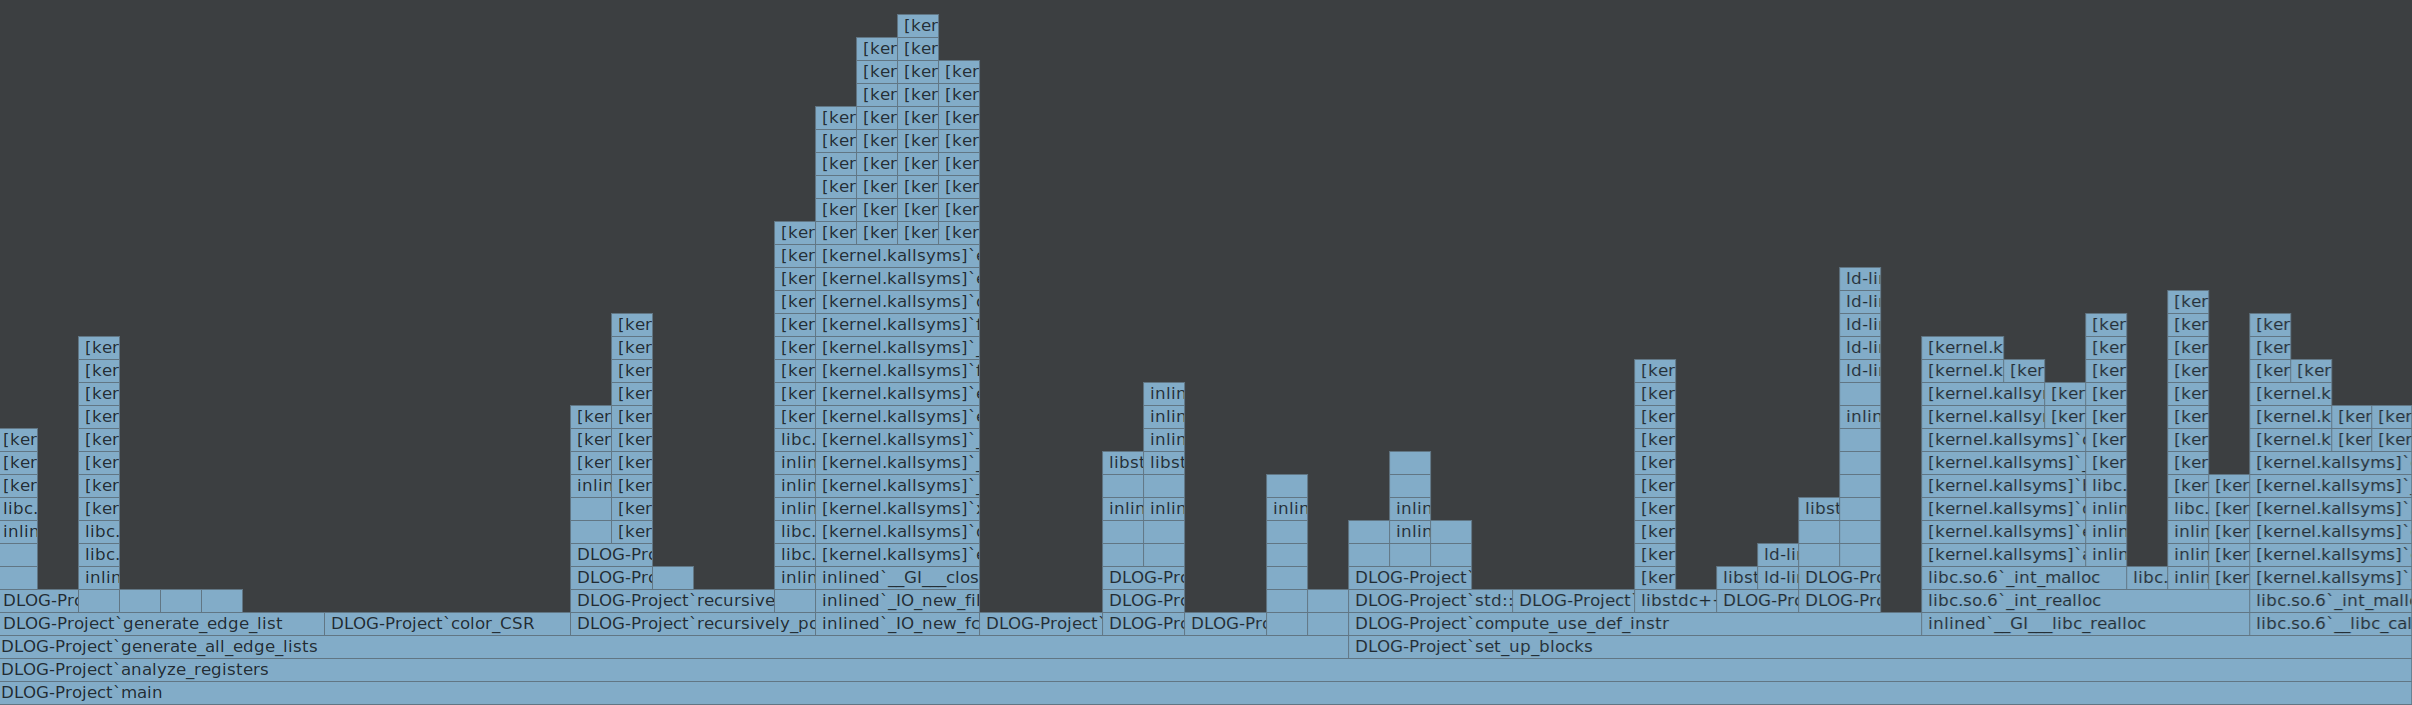
\includegraphics[width=1\linewidth]{figures/flamegraph.png}
    \caption{Flame graph, excluding I/O operations}
    \label{fig:flamegraph}
\end{figure}

Comparing our liveliness implementation and graph generator with the one developed by da Silva et. al., we found a significant improvement in execution speed. When processing larger files, the existing method seems to drastically slow down, with an equivalent processing with our method being up to 50x faster. On average, though, we saw approximately 20x speedup when processing random subsets of the FormAI dataset. This experiment was performed in a Linux terminal environment on a computer containing an Intel 12th Gen Intel(R) Core(TM) i9-12900H.

\begin{table}[H]
\centering
\caption{Time to Process Various Batches of Files}
\label{tab:batch-processing-time}
\begin{tabular}{rcc}
\toprule
\textbf{Number of Files} & \textbf{Our Method (s)} & \textbf{Baseline Method (s)} \\
\midrule
5   & 0.029 & 0.665 \\
25  & 0.066 & 2.237 \\
50  & 0.162 & 6.810 \\
100 & 0.377 & 7.086 \\
\bottomrule
\end{tabular}
\end{table}


\begin{table}[H]
\centering

\caption{Time Complexity of Relevant Algorithms }
\label{tab:bigoh}
\begin{tabular}{rcc}
\toprule
\textbf{Algorithm} & \textbf{Time Complexity} \\
\midrule
\textbf{Algorithm \ref{alg:perblock-usedef}}  & $\Theta(IR)$ \\
\textbf{Algorithm \ref{alg:phi-usedef}}  & $\Theta(\frac{P}{F}B)$ \\
\textbf{Algorithm \ref{alg:liveliness}}  & $\Theta(B\log{B})$ \\
\textbf{Algorithm \ref{alg:iggen}}  & $\Theta(IR)$ \\
\textbf{Algorithm \ref{alg:recursively-populate}}  & $\Theta(|V|^{2})$ \\
\textbf{Algorithm \ref{alg:greedy-color}}  & $\Theta(|V| + |E|)$ \\

\bottomrule

\end{tabular}
\captionsetup[sub]{font=scriptsize}
\subcaption*{*Total Blocks $(B)$, Instructions $(I)$, Vertices $(V)$, Edges $(E)$, $\phi$-nodes $(P)$, Functions $(F)$}
\end{table}



\section{Discussion}

The value of any data gathered is heavily dependent on the quality and diversity of the source code it is derived from. Examining the $\chi$ distributions, there is clearly much variety in the structure of the final output graphs, which indicates that the dataset has a lot of value in the graph features that could be learned from it. Additionally, the average $\chi$ increases by approximately one when each shallow graph is expanded. The reason this increase is so small is likely due to many of the functions having no function calls, or only calls to externally linked libraries, within. While the increase in the mean is small, a careful look at the tail of each graph reveals that there are substantially more high chromatic number graphs when functions are expanded. This indicates that deeply nested function calls introduce a lot of interference that cannot be easily solved for.

Moving on to the average degree distributions, there are some noteworthy inferences. Both the shallow and expanded graphs have a significant number of functions with 0 or extremely low average degree. This is most likely caused by a significant portion of functions containing little to no interference, as in, variable usage comes in independent sets.

Finally, the flame graph shows where there is room for improvement. Originally, we utilized cregex from the C++ STL, and that caused our graph generation process to be extremely slow. Generating a flame graph proved that those regex matches alone accounted for 99\% of the runtime. Switching to custom state machines for string matching alleviated this immensely.

\section{Conclusions}

Our project successfully addresses the current issues rooted in contemporary datasets used in graph coloring for register allocation. While current works are too theoretical or lacking in rigor, ours is capable of authentically representing the complied code, its dependencies, phi nodes, and proper liveliness. This is achieved by leveraging the full LLVM compilation pipeline along with custom passes to produce our interference graphs from real pieces of high level code. Moreover, this work can be easily extended to other languages so researchers are not boxed in to only using interference graphs of C/C++ code. The scalability of this work is validated via the successful processing of over 215,000 C files comprised of nearly 750,000 functions resulting in a high verity of graphical structures. Our custom recursive based interference graph generator accurately models interference across function calls by treating each callee as an independent subgraph. The discovery of high chromatic number graphs when functions are expanded during this processing suggests that deeply nested function calls introduce a lot of interference that cannot be easily solved for, making this data non-trivial and worth capturing for realistic register allocation scenarios. Immense performance gains, in terms of an approximate 99\% reduction in run time, were produced when we switched from regex based parsing to a custom state machine. This further validates the high scalability of our work and makes it a worthy contender to produce larger scale datasets.

\section{Future Work}

Now that we have an accurate dataset of interference graphs that are labeled with their corresponding chromatic numbers, as well as a generator that can efficiently produce as much training data as necessary, we can pursue our original goal of training a neural network model to allocate registers. This is the most obvious direction to move towards, but there are additional improvements that can be made internally as well. The simplest of which are the many areas in which execution speed could be increased. For one, the choice to use the greedy coloring algorithm was made due to its tendency to result in a lower chromatic number than other methods. However, running this algorithm in parallel is non-trivial. Exploring other coloring options, such as Jones-Plassmann, could lead to more freedom in terms of graph generation speed. Additionally, I/O operations and the minimal C++ STL features used currently comprise a significant portion of execution time. Creating a deeper level of pipeline integration that defers reads and writes to files, as well as strictly programming in C could drastically speed up the program. 

Conceptually, while we have implemented generation for multiple functions, there is a large limitation of the process, in that intermediate representation output is a compilation stage prior to linking. This means that any dynamically linked functions, as libc often is, will have no interference information available. One potential solution for this that could be explored involves generating a canonical list of interference subgraphs that can be referenced in the recursive expansion phase whenever common libc functions are called. Finally, on the hardware side of things, we could explore the different calling conventions among major CPU architectures and which registers are volatile vs nonvolatile across function calls, as well as memory spill penalties to fuel a better-tailored final register allocation that uses heuristics beyond simple coloring.

\section*{References}

\small

{
[1] O. Goudet, C. Grelier, and J.-K. Hao, “A deep learning guided memetic framework for graph coloring problems,” 2021, arXiv. doi: 10.48550/ARXIV.2109.05948.

[2] F. M. Q. Pereira, “A Survey on Register Allocation”.

[3] D. Das, S. A. Ahmad, and K. Venkataramanan, “Deep Learning-based Hybrid Graph-Coloring Algorithm for Register Allocation,” Dec. 08, 2019, arXiv: arXiv:1912.03700. doi: 10.48550/arXiv.1912.03700.

[4] B. Boissinot, S. Hack, D. Grund, B. Dupont De Dine Hin, and F. E. Rastello, “Fast liveness checking for ssa-form programs,” in Proceedings of the 6th annual IEEE/ACM international symposium on Code generation and optimization, Boston MA USA: ACM, Apr. 2008, pp. 35–44. doi: 10.1145/1356058.1356064.

[5] M. Osama, M. Truong, C. Yang, A. Buluc, and J. Owens, “Graph Coloring on the GPU,” in 2019 IEEE International Parallel and Distributed Processing Symposium Workshops (IPDPSW), Rio de Janeiro, Brazil: IEEE, May 2019, pp. 231–240. doi: 10.1109/IPDPSW.2019.00046.

[6] M. J. A. Schuetz, J. K. Brubaker, Z. Zhu, and H. G. Katzgraber, “Graph coloring with physics-inspired graph neural networks,” Phys. Rev. Research, vol. 4, no. 4, p. 043131, Nov. 2022, doi: 10.1103/PhysRevResearch.4.043131.

[7] N. Tihanyi, T. Bisztray, M. A. Ferrag, R. Jain, and L. C. Cordeiro, “How secure is AI-generated code: a large-scale comparison of large language models,” Empir Software Eng, vol. 30, no. 2, p. 47, Mar. 2025, doi: 10.1007/s10664-024-10590-1.

[8] C. Lattner and V. Adve, “LLVM: A compilation framework for lifelong program analysis \& transformation,” in International Symposium on Code Generation and Optimization, 2004. CGO 2004., San Jose, CA, USA: IEEE, 2004, pp. 75–86. doi: 10.1109/CGO.2004.1281665.

[9] D. Brélaz, “New methods to color the vertices of a graph,” Commun. ACM, vol. 22, no. 4, pp. 251–256, Apr. 1979, doi: 10.1145/359094.359101.

[10] C. Collberg, “Principles of Compilation 23: Register Allocation,” Department of Computer Science University of Arizona, 2011. Accessed: Nov. 15, 2025. [Online]. Available: https://www2.cs.arizona.edu/~collberg/Teaching/553/2011/Handouts/Handout-23.pdf

[11] G. Chaitin, “Register allocation and spilling via graph coloring,” SIGPLAN Not., vol. 39, no. 4, pp. 66–74, Apr. 2004, doi: 10.1145/989393.989403.

[12] W. Li, R. Li, Y. Ma, S. O. Chan, D. Pan, and B. Yu, “Rethinking Graph Neural Networks for the Graph Coloring Problem,” 2022, arXiv. doi: 10.48550/ARXIV.2208.06975.

[13] F. Rastello and F. Bouchez Tichadou, Eds., SSA-based Compiler Design. Cham: Springer International Publishing, 2022. doi: 10.1007/978-3-030-80515-9.

[14] P. ZAFFALON SILVA, "RigSet- UEL - Register Interference Graphs Dataset", IEEE Dataport, February 27, 2024, doi:10.21227/92af-5q05 
    
[15] D. Johnson, M. Trick, C. McGeoch, “Computational Series: Graph Coloring and its Generalizations,” Cmu.edu, 2025. https://mat.tepper.cmu.edu/COLOR02/ (accessed Dec. 13, 2025).

}

\end{document}
